\subsection{Học nhận diện địa điểm trực quan}

Để đạt hiệu quả cao trong bài toán nhận diện địa điểm trực quan, ngoài việc truy xuất được các biểu diễn đặc trưng tốt, nhiều nghiên cứu còn tập trung phát triển quá trình học truy xuất, đặt quá trình huấn luyện mô hình dưới nhiều hướng tiếp cận khác nhau. Các hướng tiếp cận này có thể được chia thành hai nhóm chính: học truy xuất thông qua phân loại và học để xếp hạng. Ngoài ra, một số nghiên cứu còn tập trung vào khả năng học từ kiến thức chuyên môn hoặc tối ưu hóa quá trình học để xếp hạng với hàm mất mát lấy cảm hứng từ phương pháp xếp hạng danh sách (listwise ranking).

\subsubsection{Học truy xuất thông qua phân loại}

Vì bài toán phân loại là một trong những bài toán đầu tiên thể hiện kết quả tốt khi áp dụng mạng nơ-ron tích chập vào quá trình trích xuất đặc trưng, các mô hình học sâu tích chập được sử dụng cho bài toán nhận diện địa điểm trực quan đầu tiên lấy cảm hứng lớn từ các mô hình phân loại thay vì các mô hình truy xuất. Các mô hình này sử dụng một mạng nơ-ron tích chập đã được huấn luyện trên tập dữ liệu ImageNet \cite{krizhevsky2012imagenet}. Học truy xuất thông qua phân loại cho phép các nhà nghiên cứu huấn luyện được các véc-tơ đặc trưng toàn cục với kích thước nhỏ, sử dụng nhãn ở cấp độ ảnh mà không cần khai phá thông tin tương quan (example mining) trong quá trình huấn luyện, dẫn tới yêu cầu tài nguyên tính toán thấp hơn đáng kể so với các mô hình hiện tại, có tiềm năng lớn trong việc mở rộng phạm vi của bài toán truy xuất lên các tập dữ liệu lớn. Đảm nhận trách nhiệm trích xuất đặc trưng biểu diễn, một số đánh giá sơ bộ cho thấy các mô hình truy xuất thông qua phân loại, mặc dù đạt kết quả tốt trong bài toán phân loại các lớp ngữ nghĩa và nhận diện ảnh ở địa danh khác nhau, không đảm bảo sẽ học được các biểu diễn đặc trưng hiệu quả cho các yếu tổ thay đổi giữa các phần từ trong một lớp, quá trình so sánh tương quan và truy xuất từ cơ sở dữ liệu \cite{arandjelovic2016netvlad, gordo2016deep, randenovic2016BoW}, thúc đẩy các nhà nghiên cứu đến các hướng tiếp cận khác. Gần đây, sự phát triển của các giải pháp phân loại ở các bài toán trích xuất đặc trưng khác đã khơi dậy lại nỗ lực nghiên cứu phương pháp này với xu hướng tăng cường khả năng học các biểu diễn đặc trưng mang tính phân biệt tốt hơn cho những yếu tố thay đổi giữa các phần tử trong cùng một lớp. Nổi bật với hai bài báo \cite{cao2020unifying, yokoo2020twostage} sử dụng hàm mất mát ArcFace \cite{Deng_2022} và tương đồng cosine để huấn luyện mô hình truy xuất thông qua phân loại, đạt kết quả tốt hơn các phương pháp truy xuất thông qua phân loại trước đó. Lấy cảm hứng từ hàm mất mát ArcFace \cite{Deng_2022}, CosPlace \cite{berton2022rethinking} tiếp tục cải tiến phương pháp truy xuất thông qua phân loại, đạt kết quả tốt nhất hiện tại cho tập dữ liệu Tokyo 24/7(Recall@5) \cite{Torii-CVPR2015} và SF-XL \cite{berton2022rethinking}. Tiếp tục phát triển từ kết quả đạt được tại CosPlace \cite{berton2022rethinking}, Berton và nnk phát triển mô hình EigenPlaces \cite{berton2023eigenplaces} đạt kết quả tốt nhất hiện tại cho tập dữ liệu AmsterTime \cite{yildiz2022amstertime}, EynSham \cite{eynsham2009}, Pittsburgh-30k-test \cite{6618963}, San Francisco Landmark \cite{5995610}, SF-XL test v1 \cite{berton2022rethinking}, Tokyo247 \cite{Torii-CVPR2015}.

\begin{figure}[H]
    \centering
    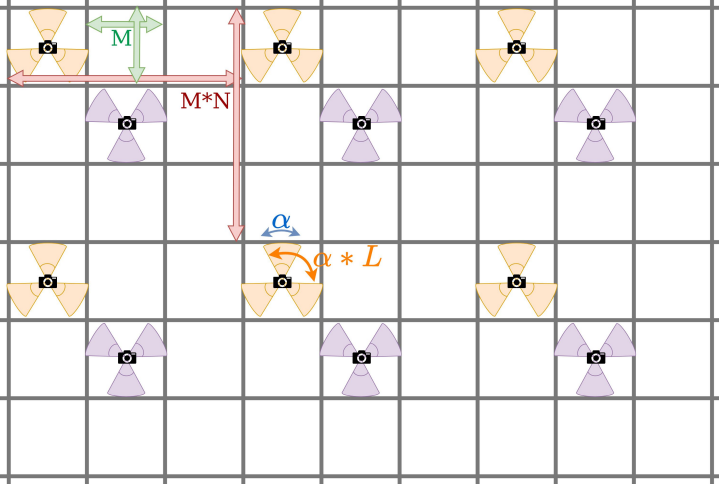
\includegraphics[width=0.7\textwidth]{pics/Chapter2/cosplaceclassify.png}
    \caption{Minh họa cách phân loại dữ liệu của mô hình CosPlace \cite{berton2022rethinking}}
\end{figure}

\subsubsection{Học truy xuất thông qua học xếp hạng}

Truy xuất hình ảnh, tương tự với bài toán "học xếp hạng", là quá trình học thông số và tìm phương thức truy xuất đặc trưng tốt nhất để biểu diễn sự tương quan giữa các phần tử trong tập dữ liệu dựa trên một hàm tính toán tương quan (distance function). Phần lớn các hướng tiếp cận cho bài toán nhận diện địa điểm trực quan sửa dụng một trong hai hàm mất mát chính với cùng ý tưởng:

\begin{itemize}
    \item hàm mất mát tương phản (contrastive loss), sử dụng các mạng nơ-ron siamese \cite{ong2017siamese, GeM, randenovic2016BoW}; và
    \item hàm mất mát ba phần tử (triplet loss), sử dụng các mạng nơ-ron có ba phần tử \cite{arandjelovic2016netvlad, gordo2016deep, gordo2017endtoend, wang2014learning, jin2017learned, zheng2018sift}.
\end{itemize}

Với mỗi mẫu dữ liệu huấn luyện, mô hình học truy xuất thông qua học xếp hạng được cung cấp những mẫu dữ liệu tích cực hoặc tiêu cực. Hàm mất mát có nhiệm vụ huấn luyện các đặc trưng sao cho những mẫu dữ liệu có giá trị tích cực sẽ có đặc trưng mang khoảng cách nhỏ và những mẫu dữ liệu có giá trị tiêu cực có khoảng cách lớn. Dưới góc nhìn của bài toán nhận diện địa điểm trực quan, một mẫu dữ liệu tích cực là ảnh ở cùng vị trí địa lý với ảnh huấn luyện, trong khi một mẫu dữ liệu tiêu cực là ảnh ở một vị trí địa lý khác. Các mô hình học truy xuất thông qua học xếp hạng có thể được chia thành hai nhóm chính: học truy xuất thông qua hàm mất mát tương phản và học truy xuất thông qua hàm mất mát ba phần tử. Như đã nhắc đến, để thực hiện quá trình học truy xuất thông qua học xếp hạng, các mô hình học truy xuất cần thực hiện quá trình khai phá thông tin tương quan (example mining) trong quá trình huấn luyện. Hướng tiếp cận này cho phép các nhà nghiên cứu phát triển các mô hình học giám sát yếu \cite{arandjelovic2016netvlad, jin2017learned} và học không giám sát \cite{radenovic2018fine} bằng cách lợi dụng các thông tin định vị để hỗ trợ quá trình khai phá. Tuy nhiên, quá trình khai phá này có chi phí tính toán cao, giới hạn thời gian và phạm vi dữ liệu có thể sử dụng để huấn luyện mô hình. \cite{arandjelovic2016netvlad} đánh dấu bước phát triển quan trọng trong hướng tiếp cận và đề xuất các hướng phát triển để tối ưu hóa quá trình này:

\begin{itemize}
    \item Lấy mẫu (Sampling): Hàm mất mát chỉ được tính cho tập hợp các mẫu dữ liệu tiêu cực và mỗi bước lấy mẫu sẽ thừa hưởng kết quả của những mẫu dữ liệu mang giá trị tiêu cực lớn nhất.
    \item Lưu đệm (Caching): Những đặc trưng được lưu trữ trong bộ nhớ đệm và chỉ được tính toán lại sau một số bước lấy mẫu huấn luyện nhất định tùy thuộc và tần suất học của mô hình (learning rate).
    \item Phân cụm (Clustering): Những đặc trưng được phân cụm dựa theo giá trị vị trí GPS thành các cụm nhỏ hơn và các mẫu huấn luyện trong cùng cụm sẽ chia sẻ cùng mẫu dữ liệu tiêu cực.
\end{itemize}
